\subsection{Основной алгоритм}
В ходе разарботки был применен видоизменнённый шаблон проектирования Factory method.

%Описание шаблона и его модификации
Данный шаблон относится к классу порождающих шаблонов. Шаблоны данного класса - это шаблоны проектирования, которые абстрагируют процесс инстанцирования (создания экземпляра класса). Они позволяют сделать систему независимой от способа создания, композиции и представления объектов. Шаблон, порождающий классы, использует наследование, чтобы изменять инстанцируемый класс, а шаблон, порождающий объекты, делегирует инстанцирование другому объекту.
Основной алгоритм представлен на рисунке \ref{architech:architech}.

\begin{figure}[h!]
\center{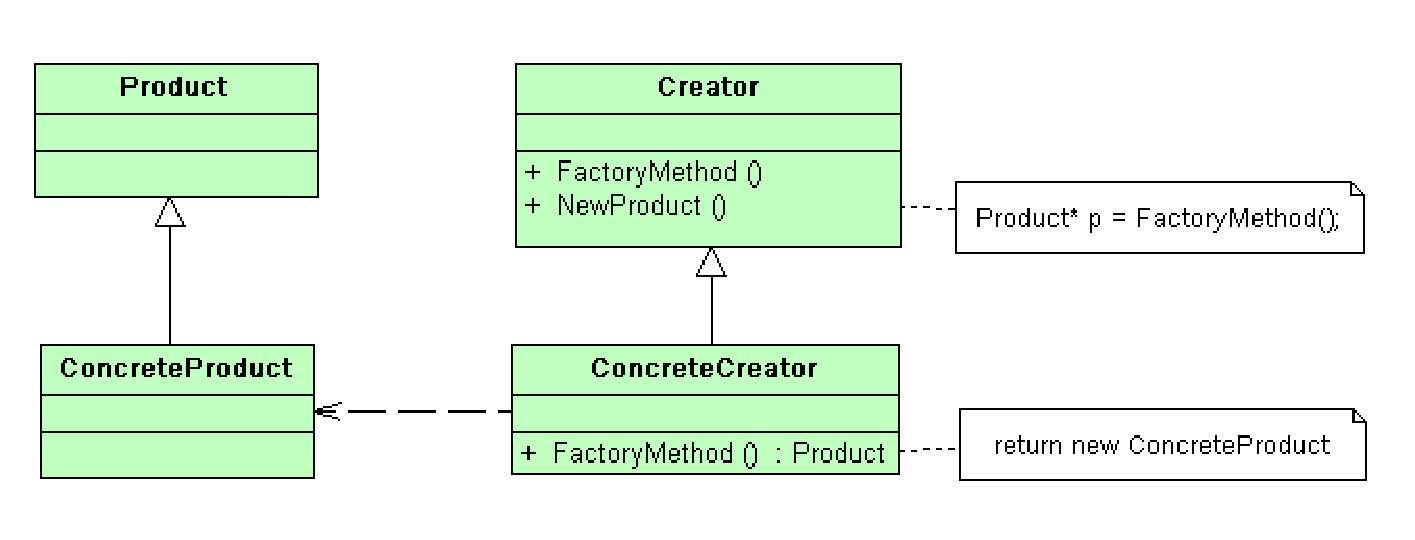
\includegraphics[width=0.9\linewidth]{architech}}
\caption{Основной алгоритм}
\label{architech:architech}
\end{figure}

Использование данного шаблона позволило нам разбить наш проект на независимые модули, что весьма упростило задачу разработки, так как написание алгоритма для конкретного таска не влияло на остальную часть проекта. При разработке был реализован базовый класс для работы с образом диска. Данный клас предназначался для формирования списка настроек, определения операционной системы на смонтированном образе и инстанционировании и накапливание всех необходимых классов-тасков в очереди тасков. После чего каждый таск из очереди отправлялся на выполнение. Блоксхема работы алгоритма (тут картинка alg_main.eps)

Каждый класс-таск порождался путем наследования от базового абстрактного класса который имеет 8 методов и 3 атрибута:

\begin{enumerate}
\item QString manual() - возвращает справку о входных параметрах данного таска;
\item void setOption(QStringList list) - установка флагов для поданных на вход параметров;
\item QString command() - возвращает команду для инициализации такска вручную;
\item bool supportOS(const coex::typeOS \&os) - возвращает флаг, указывающий на возможность использования данного таска для конкретной операционной системы;
\item QString name() - возвращает имя данного таска;
\item QString description() - возвращает краткое описание таска;
\item bool test() - предназначена для теста на доступность таска;
\item bool execute(const coex::config \&config) - запуск таска на выполнение;
\item QString m\_strName - хранит имя таска;
\item QString m\_strDescription - хранит описание таска;
\item bool m\_bDebug - флаг для параметра --debug;
\end{enumerate}

На данный момент в проекте используется восемь классов. UML-диаграмма классов представлена на рисунке (тут картинка UML.eps)

Классы taskSearchSyslogsWin, taskSearchPidginWin и taskSearchSkypeWin - наследники от класса task являются тасками. Класс winEventLog и _EVENTLOGRECORD предназначины для конвертации журнальных файлов операционной системы Windows XP, а класс writerMessages для преобразования истории переписки.